\documentclass{../../slides-style}

\slidetitleext{Лекция 11: Рефакторинг}{14.05.2024}{Рефакторинг}

\begin{document}

    \begin{frame}[plain]
        \titlepage
    \end{frame}

    \section{Введение}

    \begin{frame}
        \frametitle{Рефакторинг}
        \begin{outline}
            \1 Изменение во внутренней структуре программного обеспечения, имеющее целью облегчить понимание его работы и упростить модификацию, не затрагивая наблюдаемого поведения
                \2 Приведение кода в порядок
                \2 Изменение внешнего окружения
                \2 Борьба с деградацией архитектуры
                \2 \emph{Не} связан с оптимизацией работы кода
            \1 Декомпозиция на большое количество элементарных действий
            \1 Альтернатива проектированию архитектуры?
        \end{outline}
    \end{frame}

    \begin{frame}
        \frametitle{Зачем нужно делать рефакторинг}
        \begin{outline}
            \1 Улучшение структуры программного обеспечения
            \1 Облегчение понимания кода
            \1 Помощь в поиске ошибок
            \1 Ускорение разработки нового кода
            \1 Изменение культуры кодирования
        \end{outline}
    \end{frame}

    \section{Code smells}

    \begin{frame}
        \frametitle{Дублирование кода}
        \begin{outline}
            \1 Копипаст суть ересь
            \1 ``Выделение метода''
            \1 ``Подъём метода''
            \1 ``Выделение класса''
        \end{outline}
    \end{frame}

    \begin{frame}
        \frametitle{Длинный метод}
        \begin{outline}
            \1 Короткие методы: понятность, переиспользуемость
            \1 Усложняет чтение~--- требуется переключение контекстов
                \2 Давайте понятные имена
            \1 Семантическое расстояние между \emph{что делает код} и \emph{как}
            \1 ``Выделение метода''
            \1 Комментарии внутри тела метода~--- повод задуматься
        \end{outline}
    \end{frame}

    \begin{frame}
        \frametitle{Большой класс}
        \begin{outline}
            \1 Слишком много атрибутов
            \1 Слишком много кода
            \1 ``Выделение класса'' и ``Выделение подкласса''
        \end{outline}
    \end{frame}

    \begin{frame}
        \frametitle{Длинный список параметров}
        \begin{outline}
            \1 Сложно
            \1 Глобальные переменные нельзя, ``временные поля'' тоже нельзя
            \1 ``Выделение объекта-параметра''
        \end{outline}
    \end{frame}

    \begin{frame}
        \frametitle{Слишком много ответственностей класса}
        \begin{outline}
            \1 Single Responsibility Principle
            \1 Несколько изменений затрагивают один класс
            \1 Разделить класс на два (три, пять, и ещё один, чтобы связать их)
        \end{outline}
    \end{frame}

    \begin{frame}
        \frametitle{<<Стрельба дробью>>}
        \begin{outline}
            \1 Предыдущий ``запах'' наоборот~--- одно изменение затрагивает несколько классов
                \2 Легко пропустить важное изменение
            \1 ``Перемещение метода'' и ``Перемещение поля''
            \1 ``Встраивание класса''
        \end{outline}
    \end{frame}

    \begin{frame}
        \frametitle{<<Завистливые функции>>}
        \begin{outline}
            \1 Метод обращается к чужому классу чаще, чем к своему
            \1 ``Перемещение метода''
                \2 Плюс ``Выделение метода''
            \1 Исключение: паттерны ``Стратегия'' и ``Посетитель''
        \end{outline}
    \end{frame}

    \begin{frame}
        \frametitle{Группы данных}
        \begin{outline}
            \1 Набор значений, которые используются вместе
            \1 ``Выделение класса''
                \2 Можно вынести туда содержательную функциональность
                    \3 Найдя ``Завистливые функции''
        \end{outline}
    \end{frame}

    \begin{frame}
        \frametitle{Операторы типа switch}
        \begin{outline}
            \1 Один и тот же switch в нескольких местах программы
                \2 Легко забыть поменять кого-то из них
            \1 Коды типов
            \1 Заменить на полиморфизм
                \2 ``Выделение метода'', ``Перемещение метода''
                \2 ``Замена кода типа подклассами''
                \2 ``Заменой кода типа состоянием/стратегией''
                \2 ``Замена условного оператора полиморфизмом''
                \2 ``Введение Null-объекта''
        \end{outline}
    \end{frame}

    \begin{frame}
        \frametitle{<<Ленивый класс>>}
        \begin{outline}
            \1 Ненужный класс усложняет сопровождение
            \1 Результат рефакторинга, либо забота о будущем
            \1 ``Встраивание класса''
        \end{outline}
    \end{frame}

    \begin{frame}
        \frametitle{Временное поле}
        \begin{outline}
            \1 Атрибут, нужный только во время работы метода/передачи параметров
            \1 ``Выделение класса'', ``Введение Null-объекта''
                \2 Улучшит инкапсуляцию
        \end{outline}
    \end{frame}

    \begin{frame}[fragile]
        \frametitle{Цепочки сообщений}
        \begin{outline}
            \1 \mintinline{java}|object.getX().getY().getZ();|
            \1 ``Сокрытие делегирования''
        \end{outline}
    \end{frame}

    \begin{frame}
        \frametitle{<<Неуместная близость>>}
        \begin{outline}
            \1 Чрезмерный доступ к состоянию/private по смыслу поведению другого класса
            \1 Наследование
            \1 ``Перемещение метода'', ``Перемещение поля''
            \1 ``Выделение класса''
        \end{outline}
    \end{frame}

    \begin{frame}
        \frametitle{Классы данных}
        \begin{outline}
            \1 Только поля, геттеры и сеттеры
            \1 Не всегда плохо
            \1 ``Инкапсуляция поля'', ``Инкапсуляция коллекции''
            \1 ``Перемещение метода'', ``Выделение метода'', ``Сокрытие метода''
        \end{outline}
    \end{frame}

    \begin{frame}
        \frametitle{Комментарии}
        \begin{outline}
            \1 Код должен быть понятным и без комментариев
            \1 Комментарии могут играть роль ``дезодоранта''
            \1 \emph{Комментарии нужны}
                \2 Но должны пояснять, \emph{почему}, а не \emph{как}
            \1 ``Выделение метода''
            \1 assert-ы
        \end{outline}
    \end{frame}

    \section{Примеры рефакторингов}

    \begin{frame}[fragile]
        \frametitle{Выделение метода (Extract Method)}
        \begin{minted}{java}
void printOwing(double amount) {
    printBanner();
    // вывод деталей
    System.out.println ("name: " + _name);
    System.out.println ("amount " + amount);
}
        \end{minted}
        
        \hspace{2cm}{\Huge{$\Downarrow$}}
        
        \begin{minted}{java}
void printOwing(double amount) {
    printBanner();
    printDetails(amount);
}
void printDetails(double amount) {
    System.out.println ("name: " + _name);
    System.out.println ("amount " + amount);
}
        \end{minted}
    \end{frame}

    \begin{frame}[fragile]
        \frametitle{Встраивание метода (Inline Method)}
        \begin{minted}{java}
int getRating() {
    return moreThanFiveLateDeliveries() ? 2 : 1;
}

boolean moreThanFiveLateDeliveries() {
    return _numberOfLateDeliveries > 5;
}
        \end{minted}
        
        \hspace{2cm}{\Huge{$\Downarrow$}}
        
        \begin{minted}{java}
int getRating() {
    return _numberOfLateDeliveries > 5 ? 2 : 1;
}
        \end{minted}
    \end{frame}

    \begin{frame}[fragile]
        \frametitle{Введение поясняющей переменной}
        \begin{minted}{java}
if ((platform.toUpperCase().indexOf("MAC") > -1)
    && (browser.toUpperCase().indexOf("IE") > -1)
    && wasInitialized() && resize > 0) {

    // do something
}
        \end{minted}
        
        \hspace{2cm}{\Huge{$\Downarrow$}}
        
        \begin{minted}{java}
final boolean isMacOS = platform.toUpperCase().indexOf("MAC") > -1;
final boolean isIEBrowser = browser.toUpperCase().indexOf("IE") > -1;
final boolean isResized = resize > 0;

if (isMacOS && isIEBrowser && wasInitialized() && isResized) {
    // do something
}
        \end{minted}
    \end{frame}

    \begin{frame}[fragile]
        \frametitle{Декомпозиция условного оператора (Decompose Conditional)}
        \begin{minted}{java}
if (date.before(SUMMER_START) || date.after(SUMMER_END))
    charge = quantity * _winterRate + _winterServiceCharge;
else
    charge = quantity * _summerRate;
        \end{minted}
        
        \hspace{2cm}{\Huge{$\Downarrow$}}
        
        \begin{minted}{java}
if (notSummer(date))
    charge = winterCharge(quantity);
else
    charge = summerCharge(quantity);
        \end{minted}
    \end{frame}

    \begin{frame}[fragile]
        \frametitle{Расщепление временной переменной (Split Temporary Variable)}
        \begin{minted}{java}
double temp = 2 * (_height + _width);
System.out.println(temp);
temp = _height * _width;
System.out.println(temp);
        \end{minted}
        
        \hspace{2cm}{\Huge{$\Downarrow$}}
        
        \begin{minted}{java}
final double perimeter = 2 * (_height + _width);
System.out.println (perimeter);
final double area = _height * _width;
System.out.println (area);
        \end{minted}
    \end{frame}

    \begin{frame}[fragile]
        \frametitle{Замена метода объектом (Replace Method with Method Object)}
        \begin{footnotesize}
            \begin{minted}{java}
class Order {
    double price() {
        double primaryBasePrice;
        double secondaryBasePrice;
        double tertiaryBasePrice;
        // длинные вычисления;
    }
}
            \end{minted}
        \end{footnotesize}
        
        \hspace{5cm}{\huge{$\Downarrow$}}
        
        \begin{center}
            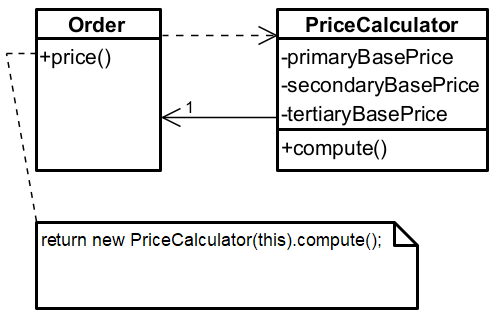
\includegraphics[width=0.4\textwidth]{methodToObject.png}
        \end{center}
    \end{frame}

    \begin{frame}
        \frametitle{Перемещение метода (Move Method)}
        \begin{center}
            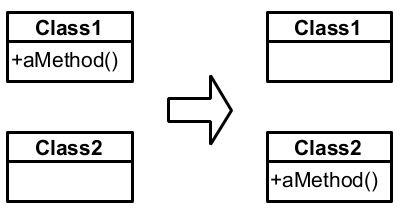
\includegraphics[width=0.4\textwidth]{moveMethod.png}
        \end{center}
    \end{frame}

    \begin{frame}
        \frametitle{Выделение класса (Extract Class)}
        \begin{center}
            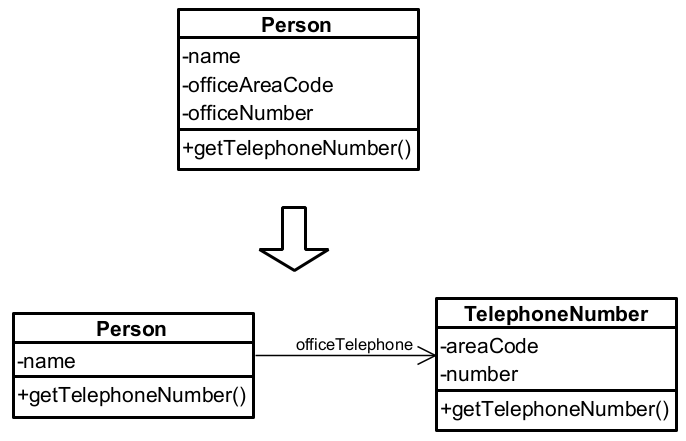
\includegraphics[width=0.7\textwidth]{extractClass.png}
        \end{center}
    \end{frame}

    \begin{frame}
        \frametitle{Сокрытие делегирования (Hide Delegate)}
        \begin{center}
            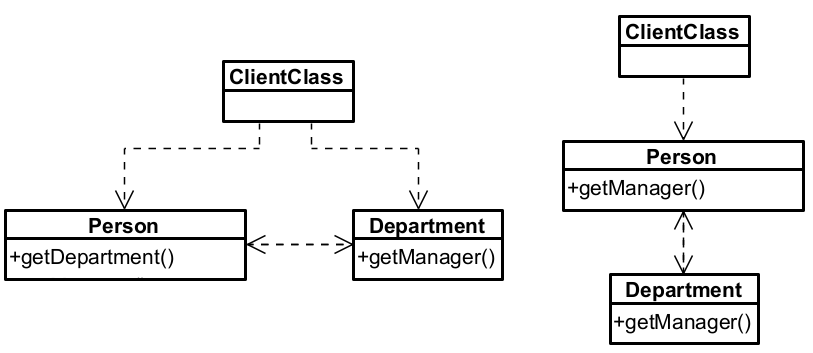
\includegraphics[width=0.8\textwidth]{hideDelegate.png}
        \end{center}
    \end{frame}

    \begin{frame}[fragile]
        \frametitle{Введение внешнего метода (Introduce Foreign Method)}
        \begin{minted}{java}
Date newStart = new Date(previousEnd.getYear(),
    previousEnd.getMonth(), previousEnd.getDate() + 1);
        \end{minted}
        
        \hspace{2cm}{\Huge{$\Downarrow$}}
        
        \begin{minted}{java}
Date newStart = nextDay(previousEnd);
static Date nextDay(Date arg) {
    return new Date (arg.getYear(), arg.getMonth(), arg.getDate() + 1);
}
        \end{minted}
    \end{frame}

    \begin{frame}[fragile]
        \frametitle{Самоинкапсуляция поля (Self Encapsulate Field)}
        \begin{minted}{java}
private int _low, _high;

boolean includes(int arg) {
    return arg >= _low && arg <= _high;
}
        \end{minted}
        
        \hspace{2cm}{\Huge{$\Downarrow$}}
        
        \begin{minted}{java}
private int _low, _high;

int getLow() { return _low; }
int getHigh() { return _high; }

boolean includes(int arg) {
    return arg >= getLow() && arg <= getHigh();
}
        \end{minted}
    \end{frame}

    \begin{frame}[fragile]
        \frametitle{Замена магического числа именованной константой}
        \begin{minted}{java}
double potentialEnergy(double mass, double height) {
    return mass * 9.81 * height;
}
        \end{minted}
        
        \hspace{2cm}{\Huge{$\Downarrow$}}
        
        \begin{minted}{java}
double potentialEnergy(double mass, double height) {
    return mass * GRAVITATIONAL_CONSTANT * height;
}

static final double GRAVITATIONAL_CONSTANT = 9.81;
        \end{minted}
    \end{frame}

    \begin{frame}
        \frametitle{Замена кода типа подклассами (Replace Type Code with Subclasses)}
        \begin{center}
            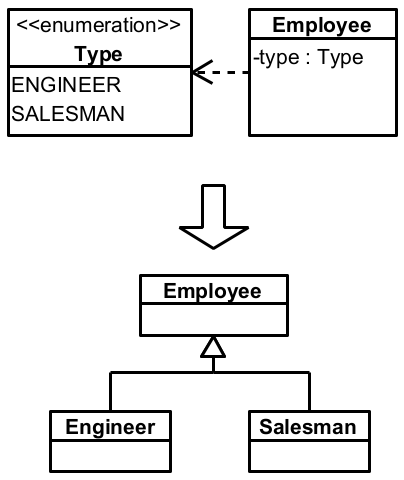
\includegraphics[width=0.4\textwidth]{replaceTypeCodeWithSubclass.png}
        \end{center}
    \end{frame}

    \begin{frame}[fragile]
        \frametitle{Замена условного оператора полиморфизмом (Replace Conditional with Polymorphism)}
        \begin{footnotesize}
            \begin{minted}{java}
double getSpeed() {
    switch (_type) {
        case EUROPEAN: return getBaseSpeed();
        case AFRICAN: return getBaseSpeed() - getLoadFactor() * _numberOfCoconuts;
        case NORWEGIAN_BLUE: return _isNailed ? 0 : getBaseSpeed(_voltage);
    }
    throw new RuntimeException("Should be unreachable");
}
            \end{minted}
        \end{footnotesize}
        
        \hspace{2cm}{\Huge{$\Downarrow$}}
        
        \begin{center}
            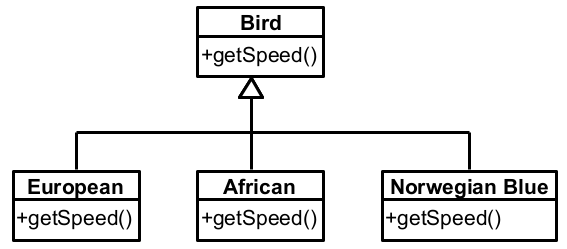
\includegraphics[width=0.5\textwidth]{replaceConditionalWithPolymorphism.png}
        \end{center}
    \end{frame}

    \begin{frame}[fragile]
        \frametitle{Введение Null-объекта (Introduce Null Object)}
        \begin{minted}{java}
if (customer == null)
    plan = BillingPlan.basic();
else
    plan = customer.getPlan();
        \end{minted}
        
        \hspace{2cm}{\Huge{$\Downarrow$}}
        
        \begin{center}
            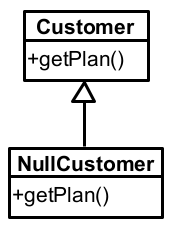
\includegraphics[width=0.15\textwidth]{nullObject.png}
        \end{center}
    \end{frame}

    \begin{frame}
        \frametitle{Разделение запроса и модификатора (Separate Query from Modifier)}
        \begin{center}
            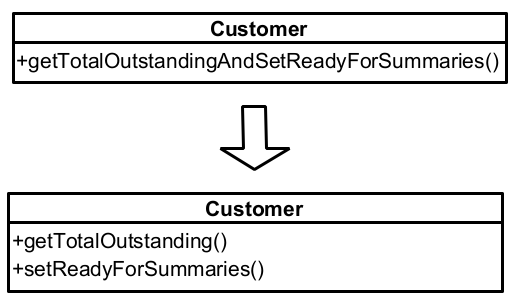
\includegraphics[width=0.5\textwidth]{separateQueryFromModifier.png}
        \end{center}
    \end{frame}

    \begin{frame}
        \frametitle{Введение объекта-параметра (Introduce Parameter Object)}
        \begin{center}
            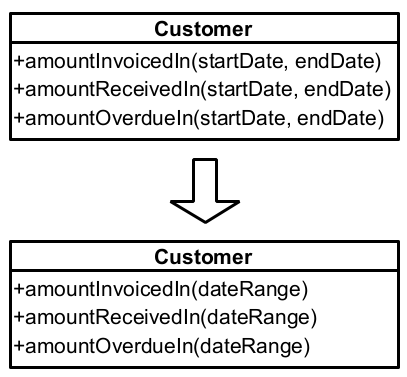
\includegraphics[width=0.4\textwidth]{introduceParameterObject.png}
        \end{center}
    \end{frame}

    \begin{frame}[fragile]
        \frametitle{Замена конструктора фабричным методом (Replace Constructor with Factory Method)}
        \begin{minted}{java}
Employee(int type) {
    _type = type;
}
        \end{minted}
        
        \hspace{2cm}{\Huge{$\Downarrow$}}
        
        \begin{minted}{java}
static Employee create(int type) {
    return new Employee(type);
}
        \end{minted}
    \end{frame}

    \begin{frame}
        \frametitle{Подъем поля (Pull Up Field)}
        \begin{center}
            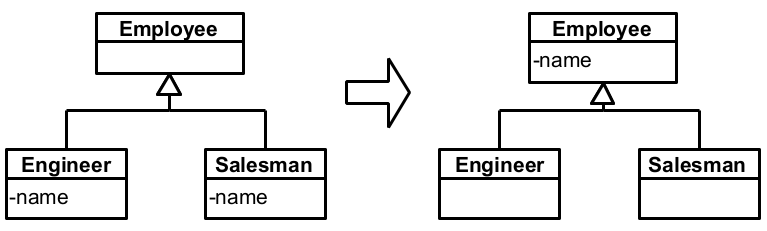
\includegraphics[width=0.8\textwidth]{pullUpField.png}
        \end{center}
    \end{frame}

    \begin{frame}
        \frametitle{Подъем метода (Pull Up Method)}
        \begin{center}
            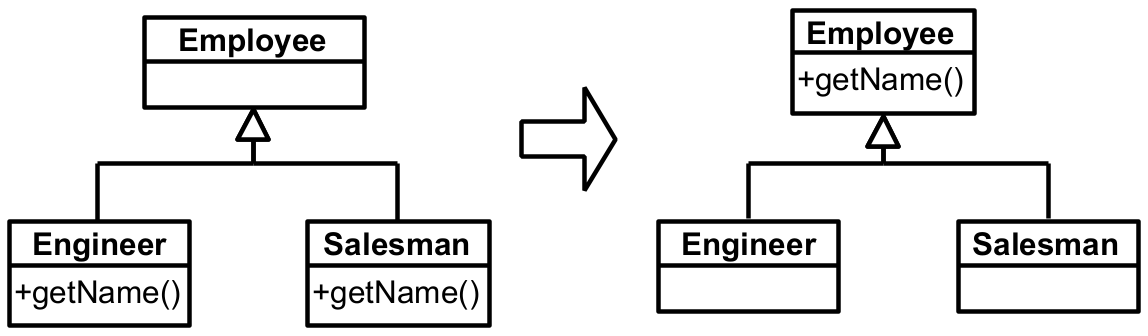
\includegraphics[width=0.8\textwidth]{pullUpMethod.png}
        \end{center}
    \end{frame}

    \begin{frame}
        \frametitle{Выделение подкласса (Extract Subclass)}
        \begin{center}
            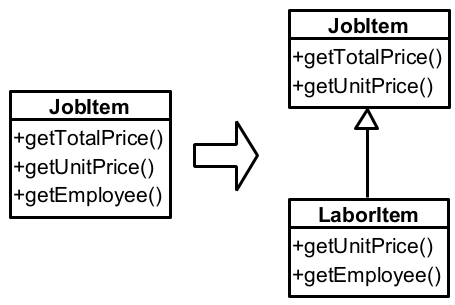
\includegraphics[width=0.4\textwidth]{extractSubclass.png}
        \end{center}
    \end{frame}

    \begin{frame}
        \frametitle{Замена наследования делегированием (Replace Inheritance with Delegation)}
        \begin{center}
            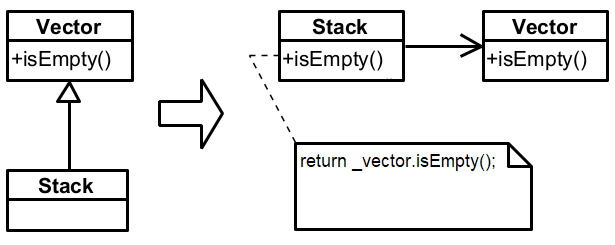
\includegraphics[width=0.7\textwidth]{replaceInheritanceWithDelegation.png}
        \end{center}
    \end{frame}

    \section{Когда делать или не делать}

    \begin{frame}
        \frametitle{Когда имеет смысл делать рефакторинг}
        \begin{outline}
            \1 Отдельное планирование
            \1 ``Правило трёх ударов''
            \1 При добавлении новой функциональности
            \1 При исправлении ошибок
            \1 При изучении и ревью кода
            \1 При устранении технического долга
        \end{outline}
    \end{frame}

    \begin{frame}
        \frametitle{Проблемы при проведении рефакторинга}
        \begin{outline}
            \1 Работа с данными
            \1 Изменение интерфейсов сущностей
                \2 Сохранение старого интерфейса
                \2 Методы-обёртки
                \2 Работа с исключениями
            \1 Глобальные изменения архитектуры
            \1 Рефакторинг и оптимизация
        \end{outline}
    \end{frame}

    \begin{frame}
        \frametitle{Когда рефакторинг делать точно не стоит}
        \begin{outline}
            \1 Код проще переписать с нуля
            \1 Близость дедлайнов
            \1 Нет юнит-тестов
        \end{outline}
    \end{frame}

    \begin{frame}
        \frametitle{Что почитать}
        \begin{center}
            
\includegraphics[width=0.9\textwidth]{books.png}
        \end{center}
    \end{frame}

\end{document}